\documentclass{article}
\usepackage{iclr2027_conference,times}
%%%%% NEW MATH DEFINITIONS %%%%%

\usepackage{amsmath,amsfonts,bm}

% Mark sections of captions for referring to divisions of figures
\newcommand{\figleft}{{\em (Left)}}
\newcommand{\figcenter}{{\em (Center)}}
\newcommand{\figright}{{\em (Right)}}
\newcommand{\figtop}{{\em (Top)}}
\newcommand{\figbottom}{{\em (Bottom)}}
\newcommand{\captiona}{{\em (a)}}
\newcommand{\captionb}{{\em (b)}}
\newcommand{\captionc}{{\em (c)}}
\newcommand{\captiond}{{\em (d)}}

% Highlight a newly defined term
\newcommand{\newterm}[1]{{\bf #1}}


% Figure reference, lower-case.
\def\figref#1{figure~\ref{#1}}
% Figure reference, capital. For start of sentence
\def\Figref#1{Figure~\ref{#1}}
\def\twofigref#1#2{figures \ref{#1} and \ref{#2}}
\def\quadfigref#1#2#3#4{figures \ref{#1}, \ref{#2}, \ref{#3} and \ref{#4}}
% Section reference, lower-case.
\def\secref#1{section~\ref{#1}}
% Section reference, capital.
\def\Secref#1{Section~\ref{#1}}
% Reference to two sections.
\def\twosecrefs#1#2{sections \ref{#1} and \ref{#2}}
% Reference to three sections.
\def\secrefs#1#2#3{sections \ref{#1}, \ref{#2} and \ref{#3}}
% Reference to an equation, lower-case.
\def\eqref#1{equation~\ref{#1}}
% Reference to an equation, upper case
\def\Eqref#1{Equation~\ref{#1}}
% A raw reference to an equation---avoid using if possible
\def\plaineqref#1{\ref{#1}}
% Reference to a chapter, lower-case.
\def\chapref#1{chapter~\ref{#1}}
% Reference to an equation, upper case.
\def\Chapref#1{Chapter~\ref{#1}}
% Reference to a range of chapters
\def\rangechapref#1#2{chapters\ref{#1}--\ref{#2}}
% Reference to an algorithm, lower-case.
\def\algref#1{algorithm~\ref{#1}}
% Reference to an algorithm, upper case.
\def\Algref#1{Algorithm~\ref{#1}}
\def\twoalgref#1#2{algorithms \ref{#1} and \ref{#2}}
\def\Twoalgref#1#2{Algorithms \ref{#1} and \ref{#2}}
% Reference to a part, lower case
\def\partref#1{part~\ref{#1}}
% Reference to a part, upper case
\def\Partref#1{Part~\ref{#1}}
\def\twopartref#1#2{parts \ref{#1} and \ref{#2}}

\def\ceil#1{\lceil #1 \rceil}
\def\floor#1{\lfloor #1 \rfloor}
\def\1{\bm{1}}
\newcommand{\train}{\mathcal{D}}
\newcommand{\valid}{\mathcal{D_{\mathrm{valid}}}}
\newcommand{\test}{\mathcal{D_{\mathrm{test}}}}

\def\eps{{\epsilon}}


% Random variables
\def\reta{{\textnormal{$\eta$}}}
\def\ra{{\textnormal{a}}}
\def\rb{{\textnormal{b}}}
\def\rc{{\textnormal{c}}}
\def\rd{{\textnormal{d}}}
\def\re{{\textnormal{e}}}
\def\rf{{\textnormal{f}}}
\def\rg{{\textnormal{g}}}
\def\rh{{\textnormal{h}}}
\def\ri{{\textnormal{i}}}
\def\rj{{\textnormal{j}}}
\def\rk{{\textnormal{k}}}
\def\rl{{\textnormal{l}}}
% rm is already a command, just don't name any random variables m
\def\rn{{\textnormal{n}}}
\def\ro{{\textnormal{o}}}
\def\rp{{\textnormal{p}}}
\def\rq{{\textnormal{q}}}
\def\rr{{\textnormal{r}}}
\def\rs{{\textnormal{s}}}
\def\rt{{\textnormal{t}}}
\def\ru{{\textnormal{u}}}
\def\rv{{\textnormal{v}}}
\def\rw{{\textnormal{w}}}
\def\rx{{\textnormal{x}}}
\def\ry{{\textnormal{y}}}
\def\rz{{\textnormal{z}}}

% Random vectors
\def\rvepsilon{{\mathbf{\epsilon}}}
\def\rvtheta{{\mathbf{\theta}}}
\def\rva{{\mathbf{a}}}
\def\rvb{{\mathbf{b}}}
\def\rvc{{\mathbf{c}}}
\def\rvd{{\mathbf{d}}}
\def\rve{{\mathbf{e}}}
\def\rvf{{\mathbf{f}}}
\def\rvg{{\mathbf{g}}}
\def\rvh{{\mathbf{h}}}
\def\rvu{{\mathbf{i}}}
\def\rvj{{\mathbf{j}}}
\def\rvk{{\mathbf{k}}}
\def\rvl{{\mathbf{l}}}
\def\rvm{{\mathbf{m}}}
\def\rvn{{\mathbf{n}}}
\def\rvo{{\mathbf{o}}}
\def\rvp{{\mathbf{p}}}
\def\rvq{{\mathbf{q}}}
\def\rvr{{\mathbf{r}}}
\def\rvs{{\mathbf{s}}}
\def\rvt{{\mathbf{t}}}
\def\rvu{{\mathbf{u}}}
\def\rvv{{\mathbf{v}}}
\def\rvw{{\mathbf{w}}}
\def\rvx{{\mathbf{x}}}
\def\rvy{{\mathbf{y}}}
\def\rvz{{\mathbf{z}}}

% Elements of random vectors
\def\erva{{\textnormal{a}}}
\def\ervb{{\textnormal{b}}}
\def\ervc{{\textnormal{c}}}
\def\ervd{{\textnormal{d}}}
\def\erve{{\textnormal{e}}}
\def\ervf{{\textnormal{f}}}
\def\ervg{{\textnormal{g}}}
\def\ervh{{\textnormal{h}}}
\def\ervi{{\textnormal{i}}}
\def\ervj{{\textnormal{j}}}
\def\ervk{{\textnormal{k}}}
\def\ervl{{\textnormal{l}}}
\def\ervm{{\textnormal{m}}}
\def\ervn{{\textnormal{n}}}
\def\ervo{{\textnormal{o}}}
\def\ervp{{\textnormal{p}}}
\def\ervq{{\textnormal{q}}}
\def\ervr{{\textnormal{r}}}
\def\ervs{{\textnormal{s}}}
\def\ervt{{\textnormal{t}}}
\def\ervu{{\textnormal{u}}}
\def\ervv{{\textnormal{v}}}
\def\ervw{{\textnormal{w}}}
\def\ervx{{\textnormal{x}}}
\def\ervy{{\textnormal{y}}}
\def\ervz{{\textnormal{z}}}

% Random matrices
\def\rmA{{\mathbf{A}}}
\def\rmB{{\mathbf{B}}}
\def\rmC{{\mathbf{C}}}
\def\rmD{{\mathbf{D}}}
\def\rmE{{\mathbf{E}}}
\def\rmF{{\mathbf{F}}}
\def\rmG{{\mathbf{G}}}
\def\rmH{{\mathbf{H}}}
\def\rmI{{\mathbf{I}}}
\def\rmJ{{\mathbf{J}}}
\def\rmK{{\mathbf{K}}}
\def\rmL{{\mathbf{L}}}
\def\rmM{{\mathbf{M}}}
\def\rmN{{\mathbf{N}}}
\def\rmO{{\mathbf{O}}}
\def\rmP{{\mathbf{P}}}
\def\rmQ{{\mathbf{Q}}}
\def\rmR{{\mathbf{R}}}
\def\rmS{{\mathbf{S}}}
\def\rmT{{\mathbf{T}}}
\def\rmU{{\mathbf{U}}}
\def\rmV{{\mathbf{V}}}
\def\rmW{{\mathbf{W}}}
\def\rmX{{\mathbf{X}}}
\def\rmY{{\mathbf{Y}}}
\def\rmZ{{\mathbf{Z}}}

% Elements of random matrices
\def\ermA{{\textnormal{A}}}
\def\ermB{{\textnormal{B}}}
\def\ermC{{\textnormal{C}}}
\def\ermD{{\textnormal{D}}}
\def\ermE{{\textnormal{E}}}
\def\ermF{{\textnormal{F}}}
\def\ermG{{\textnormal{G}}}
\def\ermH{{\textnormal{H}}}
\def\ermI{{\textnormal{I}}}
\def\ermJ{{\textnormal{J}}}
\def\ermK{{\textnormal{K}}}
\def\ermL{{\textnormal{L}}}
\def\ermM{{\textnormal{M}}}
\def\ermN{{\textnormal{N}}}
\def\ermO{{\textnormal{O}}}
\def\ermP{{\textnormal{P}}}
\def\ermQ{{\textnormal{Q}}}
\def\ermR{{\textnormal{R}}}
\def\ermS{{\textnormal{S}}}
\def\ermT{{\textnormal{T}}}
\def\ermU{{\textnormal{U}}}
\def\ermV{{\textnormal{V}}}
\def\ermW{{\textnormal{W}}}
\def\ermX{{\textnormal{X}}}
\def\ermY{{\textnormal{Y}}}
\def\ermZ{{\textnormal{Z}}}

% Vectors
\def\vzero{{\bm{0}}}
\def\vone{{\bm{1}}}
\def\vmu{{\bm{\mu}}}
\def\vtheta{{\bm{\theta}}}
\def\va{{\bm{a}}}
\def\vb{{\bm{b}}}
\def\vc{{\bm{c}}}
\def\vd{{\bm{d}}}
\def\ve{{\bm{e}}}
\def\vf{{\bm{f}}}
\def\vg{{\bm{g}}}
\def\vh{{\bm{h}}}
\def\vi{{\bm{i}}}
\def\vj{{\bm{j}}}
\def\vk{{\bm{k}}}
\def\vl{{\bm{l}}}
\def\vm{{\bm{m}}}
\def\vn{{\bm{n}}}
\def\vo{{\bm{o}}}
\def\vp{{\bm{p}}}
\def\vq{{\bm{q}}}
\def\vr{{\bm{r}}}
\def\vs{{\bm{s}}}
\def\vt{{\bm{t}}}
\def\vu{{\bm{u}}}
\def\vv{{\bm{v}}}
\def\vw{{\bm{w}}}
\def\vx{{\bm{x}}}
\def\vy{{\bm{y}}}
\def\vz{{\bm{z}}}

% Elements of vectors
\def\evalpha{{\alpha}}
\def\evbeta{{\beta}}
\def\evepsilon{{\epsilon}}
\def\evlambda{{\lambda}}
\def\evomega{{\omega}}
\def\evmu{{\mu}}
\def\evpsi{{\psi}}
\def\evsigma{{\sigma}}
\def\evtheta{{\theta}}
\def\eva{{a}}
\def\evb{{b}}
\def\evc{{c}}
\def\evd{{d}}
\def\eve{{e}}
\def\evf{{f}}
\def\evg{{g}}
\def\evh{{h}}
\def\evi{{i}}
\def\evj{{j}}
\def\evk{{k}}
\def\evl{{l}}
\def\evm{{m}}
\def\evn{{n}}
\def\evo{{o}}
\def\evp{{p}}
\def\evq{{q}}
\def\evr{{r}}
\def\evs{{s}}
\def\evt{{t}}
\def\evu{{u}}
\def\evv{{v}}
\def\evw{{w}}
\def\evx{{x}}
\def\evy{{y}}
\def\evz{{z}}

% Matrix
\def\mA{{\bm{A}}}
\def\mB{{\bm{B}}}
\def\mC{{\bm{C}}}
\def\mD{{\bm{D}}}
\def\mE{{\bm{E}}}
\def\mF{{\bm{F}}}
\def\mG{{\bm{G}}}
\def\mH{{\bm{H}}}
\def\mI{{\bm{I}}}
\def\mJ{{\bm{J}}}
\def\mK{{\bm{K}}}
\def\mL{{\bm{L}}}
\def\mM{{\bm{M}}}
\def\mN{{\bm{N}}}
\def\mO{{\bm{O}}}
\def\mP{{\bm{P}}}
\def\mQ{{\bm{Q}}}
\def\mR{{\bm{R}}}
\def\mS{{\bm{S}}}
\def\mT{{\bm{T}}}
\def\mU{{\bm{U}}}
\def\mV{{\bm{V}}}
\def\mW{{\bm{W}}}
\def\mX{{\bm{X}}}
\def\mY{{\bm{Y}}}
\def\mZ{{\bm{Z}}}
\def\mBeta{{\bm{\beta}}}
\def\mPhi{{\bm{\Phi}}}
\def\mLambda{{\bm{\Lambda}}}
\def\mSigma{{\bm{\Sigma}}}

% Tensor
\DeclareMathAlphabet{\mathsfit}{\encodingdefault}{\sfdefault}{m}{sl}
\SetMathAlphabet{\mathsfit}{bold}{\encodingdefault}{\sfdefault}{bx}{n}
\newcommand{\tens}[1]{\bm{\mathsfit{#1}}}
\def\tA{{\tens{A}}}
\def\tB{{\tens{B}}}
\def\tC{{\tens{C}}}
\def\tD{{\tens{D}}}
\def\tE{{\tens{E}}}
\def\tF{{\tens{F}}}
\def\tG{{\tens{G}}}
\def\tH{{\tens{H}}}
\def\tI{{\tens{I}}}
\def\tJ{{\tens{J}}}
\def\tK{{\tens{K}}}
\def\tL{{\tens{L}}}
\def\tM{{\tens{M}}}
\def\tN{{\tens{N}}}
\def\tO{{\tens{O}}}
\def\tP{{\tens{P}}}
\def\tQ{{\tens{Q}}}
\def\tR{{\tens{R}}}
\def\tS{{\tens{S}}}
\def\tT{{\tens{T}}}
\def\tU{{\tens{U}}}
\def\tV{{\tens{V}}}
\def\tW{{\tens{W}}}
\def\tX{{\tens{X}}}
\def\tY{{\tens{Y}}}
\def\tZ{{\tens{Z}}}


% Graph
\def\gA{{\mathcal{A}}}
\def\gB{{\mathcal{B}}}
\def\gC{{\mathcal{C}}}
\def\gD{{\mathcal{D}}}
\def\gE{{\mathcal{E}}}
\def\gF{{\mathcal{F}}}
\def\gG{{\mathcal{G}}}
\def\gH{{\mathcal{H}}}
\def\gI{{\mathcal{I}}}
\def\gJ{{\mathcal{J}}}
\def\gK{{\mathcal{K}}}
\def\gL{{\mathcal{L}}}
\def\gM{{\mathcal{M}}}
\def\gN{{\mathcal{N}}}
\def\gO{{\mathcal{O}}}
\def\gP{{\mathcal{P}}}
\def\gQ{{\mathcal{Q}}}
\def\gR{{\mathcal{R}}}
\def\gS{{\mathcal{S}}}
\def\gT{{\mathcal{T}}}
\def\gU{{\mathcal{U}}}
\def\gV{{\mathcal{V}}}
\def\gW{{\mathcal{W}}}
\def\gX{{\mathcal{X}}}
\def\gY{{\mathcal{Y}}}
\def\gZ{{\mathcal{Z}}}

% Sets
\def\sA{{\mathbb{A}}}
\def\sB{{\mathbb{B}}}
\def\sC{{\mathbb{C}}}
\def\sD{{\mathbb{D}}}
% Don't use a set called E, because this would be the same as our symbol
% for expectation.
\def\sF{{\mathbb{F}}}
\def\sG{{\mathbb{G}}}
\def\sH{{\mathbb{H}}}
\def\sI{{\mathbb{I}}}
\def\sJ{{\mathbb{J}}}
\def\sK{{\mathbb{K}}}
\def\sL{{\mathbb{L}}}
\def\sM{{\mathbb{M}}}
\def\sN{{\mathbb{N}}}
\def\sO{{\mathbb{O}}}
\def\sP{{\mathbb{P}}}
\def\sQ{{\mathbb{Q}}}
\def\sR{{\mathbb{R}}}
\def\sS{{\mathbb{S}}}
\def\sT{{\mathbb{T}}}
\def\sU{{\mathbb{U}}}
\def\sV{{\mathbb{V}}}
\def\sW{{\mathbb{W}}}
\def\sX{{\mathbb{X}}}
\def\sY{{\mathbb{Y}}}
\def\sZ{{\mathbb{Z}}}

% Entries of a matrix
\def\emLambda{{\Lambda}}
\def\emA{{A}}
\def\emB{{B}}
\def\emC{{C}}
\def\emD{{D}}
\def\emE{{E}}
\def\emF{{F}}
\def\emG{{G}}
\def\emH{{H}}
\def\emI{{I}}
\def\emJ{{J}}
\def\emK{{K}}
\def\emL{{L}}
\def\emM{{M}}
\def\emN{{N}}
\def\emO{{O}}
\def\emP{{P}}
\def\emQ{{Q}}
\def\emR{{R}}
\def\emS{{S}}
\def\emT{{T}}
\def\emU{{U}}
\def\emV{{V}}
\def\emW{{W}}
\def\emX{{X}}
\def\emY{{Y}}
\def\emZ{{Z}}
\def\emSigma{{\Sigma}}

% entries of a tensor
% Same font as tensor, without \bm wrapper
\newcommand{\etens}[1]{\mathsfit{#1}}
\def\etLambda{{\etens{\Lambda}}}
\def\etA{{\etens{A}}}
\def\etB{{\etens{B}}}
\def\etC{{\etens{C}}}
\def\etD{{\etens{D}}}
\def\etE{{\etens{E}}}
\def\etF{{\etens{F}}}
\def\etG{{\etens{G}}}
\def\etH{{\etens{H}}}
\def\etI{{\etens{I}}}
\def\etJ{{\etens{J}}}
\def\etK{{\etens{K}}}
\def\etL{{\etens{L}}}
\def\etM{{\etens{M}}}
\def\etN{{\etens{N}}}
\def\etO{{\etens{O}}}
\def\etP{{\etens{P}}}
\def\etQ{{\etens{Q}}}
\def\etR{{\etens{R}}}
\def\etS{{\etens{S}}}
\def\etT{{\etens{T}}}
\def\etU{{\etens{U}}}
\def\etV{{\etens{V}}}
\def\etW{{\etens{W}}}
\def\etX{{\etens{X}}}
\def\etY{{\etens{Y}}}
\def\etZ{{\etens{Z}}}

% The true underlying data generating distribution
\newcommand{\pdata}{p_{\rm{data}}}
% The empirical distribution defined by the training set
\newcommand{\ptrain}{\hat{p}_{\rm{data}}}
\newcommand{\Ptrain}{\hat{P}_{\rm{data}}}
% The model distribution
\newcommand{\pmodel}{p_{\rm{model}}}
\newcommand{\Pmodel}{P_{\rm{model}}}
\newcommand{\ptildemodel}{\tilde{p}_{\rm{model}}}
% Stochastic autoencoder distributions
\newcommand{\pencode}{p_{\rm{encoder}}}
\newcommand{\pdecode}{p_{\rm{decoder}}}
\newcommand{\precons}{p_{\rm{reconstruct}}}

\newcommand{\laplace}{\mathrm{Laplace}} % Laplace distribution

\newcommand{\E}{\mathbb{E}}
\newcommand{\Ls}{\mathcal{L}}
\newcommand{\R}{\mathbb{R}}
\newcommand{\emp}{\tilde{p}}
\newcommand{\lr}{\alpha}
\newcommand{\reg}{\lambda}
\newcommand{\rect}{\mathrm{rectifier}}
\newcommand{\softmax}{\mathrm{softmax}}
\newcommand{\sigmoid}{\sigma}
\newcommand{\softplus}{\zeta}
\newcommand{\KL}{D_{\mathrm{KL}}}
\newcommand{\Var}{\mathrm{Var}}
\newcommand{\standarderror}{\mathrm{SE}}
\newcommand{\Cov}{\mathrm{Cov}}
% Wolfram Mathworld says $L^2$ is for function spaces and $\ell^2$ is for vectors
% But then they seem to use $L^2$ for vectors throughout the site, and so does
% wikipedia.
\newcommand{\normlzero}{L^0}
\newcommand{\normlone}{L^1}
\newcommand{\normltwo}{L^2}
\newcommand{\normlp}{L^p}
\newcommand{\normmax}{L^\infty}

\newcommand{\parents}{Pa} % See usage in notation.tex. Chosen to match Daphne's book.

\DeclareMathOperator*{\argmax}{arg\,max}
\DeclareMathOperator*{\argmin}{arg\,min}

\DeclareMathOperator{\sign}{sign}
\DeclareMathOperator{\Tr}{Tr}
\let\ab\allowbreak

\usepackage{graphicx}
\usepackage{booktabs}
\usepackage{tabularx}
\usepackage{xcolor}
\usepackage{hyperref}
\usepackage{url}

\title{Constructed Negatives Shape the Evaluation of Sequence-Based Protein--Protein Interaction Models}
% Anonymous submission. Keep \iclrfinalcopy commented.
%\iclrfinalcopy
\author{Anonymous Authors}

\graphicspath{{../figures/e003_negative_representation/}{../figures/e003_final/}{../figures/iclr2027_final/}}

\begin{document}
\maketitle

\begin{abstract}
Sequence-based protein--protein interaction (PPI) models are often trained and
evaluated using unobserved protein pairs as negatives because experimentally
established non-interactions are scarce. We test how this choice affects model
evaluation. PPIShift trains four sequence-based models with six negative
constructions and evaluates each trained model against all six test-negative
constructions, giving 432 Gold evaluations while keeping the positive pairs,
class balance, sequence subset, and validation procedure fixed. For Frozen-ESM2
and TUnA, changing only the test negatives changes AUPRC by up to 0.264 and
0.249, respectively. Changing the training negatives also changes performance
and model ordering. In a within-class partner-shuffling control, shuffling
partners on the ESM-matched test set \emph{increases} AUROC by 0.086 for both
Frozen-ESM2 and TUnA even though the original protein pairs are broken. On
independent Vidal/Y2H and IntAct measurements, AUROC varies by as much as 0.193
across training-negative constructions without retraining or external
selection. Negative construction can therefore change how difficult the
benchmark is, which simple signals are predictive, whether the score depends on
the original pair, and how models perform on measured assays. Reported PPI
performance is conditional on how the negative class is constructed.
\end{abstract}

\section{Introduction}

Protein--protein interaction prediction is often formulated as binary
classification from two protein sequences. Positive examples can be collected
from interaction databases and systematic assays, but experimentally
established non-interactions are much rarer. Large supervised datasets
therefore usually construct the negative class from protein pairs that have not
been observed to interact.

This choice changes the task. A negative generator can change protein degree,
sequence length or composition, functional relatedness, taxonomic identity,
representation-space distance, endpoint frequency, and other properties. A
classifier can exploit any property associated with the label, even when that
property does not encode compatibility of the specific protein pair.
Negative-set design can therefore make PPI classification artificially easy
\citep{benhur2006}; training and evaluation negatives serve different purposes
\citep{park2011}; and protein reuse or sequence similarity can invalidate
pair-input generalization claims \citep{park2012,bernett2024}. Recent work has
also identified taxonomic, representation-level, and dataset-construction
shortcuts \citep{hallee2026,szymborski2026,bernett2026}.

This leads to a direct question: \emph{do conclusions about a model remain the
same when negative construction changes?} Existing studies often change one
sampler, one split, or one model at a time. That makes it difficult to separate
the effect of training negatives from the effect of test negatives, or to tell
whether reducing a benchmark shortcut improves transfer.

We introduce \textbf{PPIShift}, a controlled experiment that varies negative
construction independently at training and evaluation. The positive pairs,
protein-disjoint Gold split, class balance, common 512-residue sequence subset,
model-selection procedure, and random seeds are fixed. Four sequence-based
models are trained with six negative constructions, and every trained model is
evaluated unchanged on all six test-negative constructions. We also test simple
property-based, protein-only, pooled-ESM, and partner-shuffling controls, then
score the same models on independent measured datasets and an official
DataSAIL split.

We find four patterns. First, both absolute performance and model ordering
change with the negative construction. Second, reducing one shortcut does not
remove all simple predictive signals. Third, some models retain discrimination after the original A--B pairing is
broken. Fourth, the
training-negative construction still affects performance on independent
measured datasets. These properties should be evaluated separately.

Our contributions are:
\begin{enumerate}
  \item a complete training-negative $\times$ test-negative experiment over
  four sequence-based PPI models and six negative constructions;
  \item direct tests of label predictability without the original protein pair,
  including partner-shuffled evaluation of trained models;
  \item evaluation of the same trained models on measured Vidal/Y2H and IntAct
  outcomes, external BioGRID/STRING datasets, and an official DataSAIL split;
  \item a reproducibility package with fixed evaluation definitions,
  machine-readable figure data, sampler/model fidelity audits, and explicit
  label definitions for constructed and measured negatives.
\end{enumerate}

\section{Related Work}

\paragraph{Negative construction.}
Negative sampling has long been known to affect PPI evaluation.
\citet{benhur2006} showed that biologically motivated non-colocalized negatives
can create an easier feature distribution. \citet{park2011} distinguished the
requirements of negative sampling for model training from those of performance
estimation. More recent work proposed degree-balanced, similarity-aware, and
topology-driven negatives. Li et al. show that random negatives in scale-free
biomolecular networks can make node degree predictive and propose
degree-distribution-balanced sampling \citep{li2025ddb}. TPPNI combines a
configuration-model criterion with Contrastive-L3 filtering
\citep{chatterjee2025}. We use these methods as comparison conditions; the
negative-generation methods themselves are not our contribution.

\paragraph{Leakage and shortcut auditing.}
Protein and sequence overlap are established failure modes for pair-input
benchmarks \citep{park2012,bernett2024}. DataSAIL provides similarity-aware
splitting for biological machine learning \citep{joeres2025}; its 2026 addendum
evaluates the Bernett Gold PPI split \citep{joeres2026addendum}. Pretrained
protein language models can also carry prior PPI exposure
\citep{szymborski2026}. In multi-species data, taxonomy can itself become a
negative-sampling shortcut \citep{hallee2026}. These studies address different
problems: split leakage, exposure during representation pretraining, negative
construction, and dataset shift.

The most directly related work is \citet{bernett2026}, which audits topology,
self-interaction, taxonomy, functional relatedness, sequence, and
embedding-associated shortcuts and proposes similarity-aware splitting plus
bias-minimizing ILP negative sampling. We instead vary training and test
negatives independently and ask whether model comparisons, pair dependence,
and transfer change with that choice.

\paragraph{Sequence-based models.}
We evaluate a simple Frozen-ESM2 pair MLP together with three published
architectures whose implementations were checked against their source code and
methods: TUnA
\citep{ko2024}, RAPPPID \citep{szymborski2022}, and the ESM2-based D-SCRIPT
implementation evaluated by \citet{reim2025}. The original D-SCRIPT architecture
is from \citet{sledzieski2021}. ESM2 provides the frozen protein
representations used by several models and controls \citep{lin2023esm2}.

\section{Data and Experimental Design}

\subsection{Gold benchmark and common sequence subset}

We use the human Gold benchmark of \citet{bernett2024}, subsequently used by
\citet{reim2025}. Its released train, validation, and test splits are
protein-disjoint. To evaluate all four models without sequence cropping, we use
a maximum sequence length of 512 residues. This retains 13,304 training
positives, 11,085 validation positives, and 10,111 test positives. Only 16.3\%
of the original Gold training positives remain, so the main results apply to
this sequence-compatible subset.

Each negative construction contains one constructed negative per positive.
Across the six Gold test sets, the positive pairs are identical; only the
negative pairs change. We call constructed negatives \emph{synthetic unobserved
pairs}. A pair that is absent from the positive registry under our exclusion
rules is not necessarily a biological non-interaction.

\subsection{Six negative constructions}

We compare six constructions. \textbf{Uniform} samples an eligible partner
without property matching. \textbf{Degree-matched} matches train-visible
endpoint degree. \textbf{Sequence-matched} reduces differences in predefined
sequence features, and \textbf{ESM-matched} selects partners close in frozen
ESM2 space. \textbf{Bernett 2026} is our audited implementation of the
bias-reducing ILP sampler of \citet{bernett2026}. \textbf{TPPNI (balanced)} is
a fixed-size balanced set generated with the audited TPPNI topology pipeline
\citep{chatterjee2025}. In the protein-disjoint Gold test set, train-visible
degree has no useful variation, so the degree-matched test condition is kept
only as a diagnostic.

\begin{figure*}[t]
  \centering
  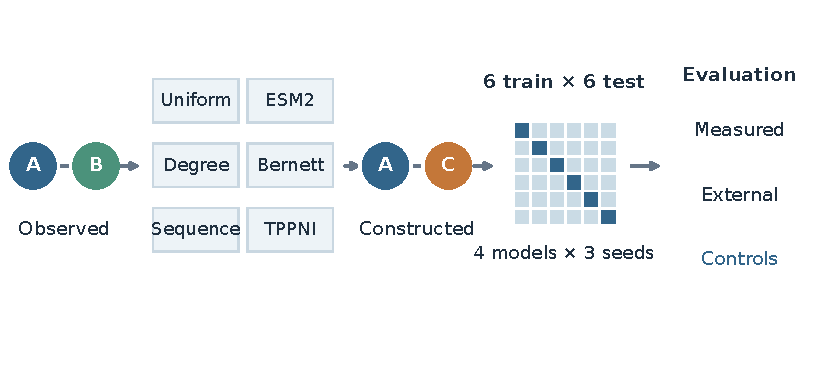
\includegraphics[width=\textwidth]{figure_01_negative_construction_explainer.pdf}
  \caption{\textbf{From an observed positive to factorial and external
  evaluations.} Starting from an observed positive pair $A$--$B$, each of six
  predeclared constructions replaces partner $B$ with $C$, producing a
  synthetic unobserved pair $A$--$C$. This label does not establish a biological
  non-interaction. The Gold factorial crosses six training-negative with six
  test-negative constructions for four models and seeds 11, 22, and 33. Models
  are also scored on measured Vidal/Y2H and IntAct outcomes, controlled BioGRID
  and STRING surfaces, and shortcut controls without external-driven retraining
  or model selection. Train-visible degree matching on the protein-disjoint
  Gold test set is degenerate and is retained as a diagnostic.}
  \label{fig:construction}
\end{figure*}

\subsection{Models, training, and model selection}

We evaluate Frozen-ESM2 pair MLP, D-SCRIPT-ESM2, RAPPPID, and corrected TUnA.
Each model is trained with each of the six negative constructions using seeds
11, 22, and 33, giving 72 trained model instances. Every trained model is then evaluated on all six fixed Gold test sets, giving
432 evaluations. Of these, 216 are newly computed; the other 216 reuse exact
scores from an earlier compatible run after hash verification.

Checkpoint selection, early stopping, thresholds, and calibration choices are
determined using validation data only. Test and external labels are not used
for training, model selection, sampler fitting, or model inclusion. On balanced
Gold test sets, AUPRC is the primary classification metric and AUROC is also
reported.

\subsection{Evaluation on measured and leakage-reduced datasets}

We score all Gold-trained models, without retraining or adaptation, on a fixed
sequence-compatible Vidal/Lambourne Y2H set containing 846 detected
interactions and 3,185 assay non-detections \citep{lambourne2026}, and on an
IntAct set containing 10,111 positives and 236 explicit curated negatives.
Assay non-detections and curated negatives are kept distinct from synthetic
unobserved pairs. We also evaluate cross-source BioGRID and STRING positive
pairs with controlled constructed negatives.

Separately, we evaluate three models on the published leakage-reduced DataSAIL
split. We use \emph{cross-source} only when the data source changes and reserve
\emph{strict OOD} for comparisons with an explicit separation criterion
relative to training.

\subsection{Shortcut and pair-dependence controls}

We use four controls. The \textbf{easy-property} classifier uses predefined
dataset features such as degree and sequence statistics. A
\textbf{single-protein sequence} classifier predicts the pair label from
single-protein sequence information without representing the A--B relation. A
\textbf{simple pooled-ESM} classifier tests whether a small classifier can
separate labels from pooled ESM representations. Finally,
\textbf{partner-shuffled evaluation} keeps the trained PPI model fixed and
permutes the second protein within each label class. This preserves label
counts and the single-protein distributions but breaks the original protein
pairs.

\section{Results}

\subsection{Negative construction changes performance and model ordering}

With Uniform negatives for both training and testing, mean AUPRC is 0.723 for
TUnA, 0.697 for Frozen-ESM2, 0.587 for D-SCRIPT-ESM2, and 0.518 for RAPPPID.
These values change when the negative construction changes. Holding the trained
model fixed and changing only the test negatives gives an average AUPRC range
of 0.165 for TUnA and 0.147 for Frozen-ESM2, with maximum ranges of 0.249 and
0.264. Holding the test set fixed and changing only the training negatives gives an
average AUPRC range of 0.138 for TUnA and 0.109 for Frozen-ESM2. D-SCRIPT and
RAPPPID also vary across constructions.

\begin{figure*}[t]
  \centering
  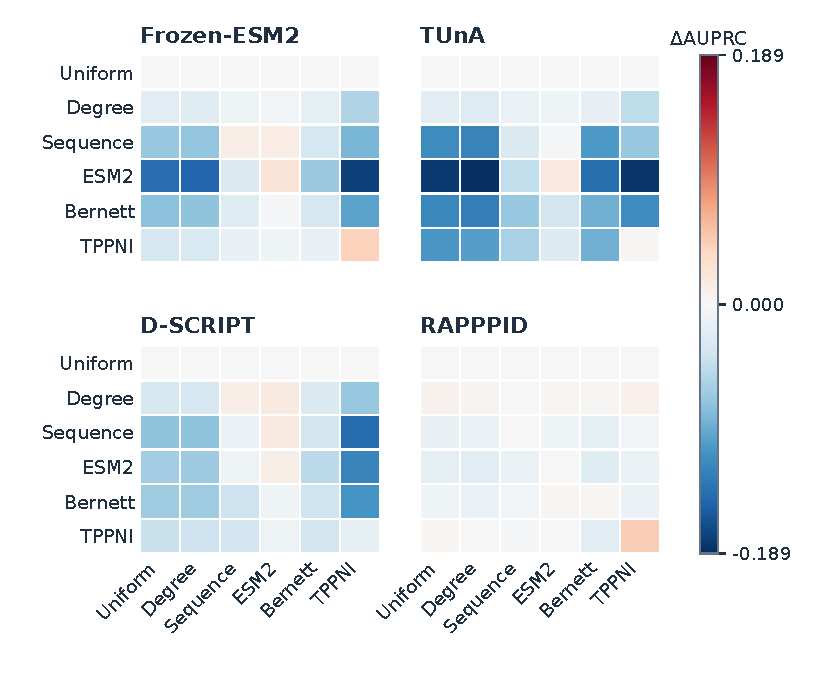
\includegraphics[width=\textwidth]{figure_02_negative_transfer.pdf}
  \caption{\textbf{Training and test negative construction both change
  performance.} Each panel shows one model on the six-by-six Gold factorial;
  rows are training-negative constructions and columns are test-negative
  constructions. Cell color shows the mean AUPRC difference from Uniform
  training on the same test-negative construction, averaged over seeds 11, 22,
  and 33; exact values are in the source table. The Uniform-training row is zero
  by definition. These
  constructed negatives are synthetic unobserved pairs, not verified biological
  non-interactions.}
  \label{fig:factorial}
\end{figure*}

Model order also changes. Over the 36 train-by-test settings, Frozen-ESM2 has
the highest mean AUPRC in 20, TUnA in 15, D-SCRIPT-ESM2 in one, and RAPPPID in
none. Across 3,780 eligible model-pair comparisons, 290 change ordering
(16.88\%); 178 are also supported by paired evaluation resampling and
seed-to-seed consistency (4.71\%). These percentages summarize the tested
settings and do not define a universal model ranking.

Matching the training and test negative construction does not consistently
improve performance. Some matched conditions improve over Uniform training,
while others decrease. Negative construction therefore cannot be summarized by
a single notion of task difficulty.

\subsection{Different negative constructions leave different shortcut signals}

The controls show that reducing one shortcut does not remove all simple
predictive signals. On the Gold test set built with Bernett negatives, the
easy-property classifier is close to chance (AUROC 0.514), consistent with the
features targeted by that construction being better matched. On the
TPPNI-balanced test set, however, a single-protein sequence classifier reaches
AUROC 0.648 and the simple pooled-ESM classifier reaches 0.669.

A negative set cannot be summarized as simply biased or unbiased. Different
negative constructions change which simple features distinguish positives from
negatives.

\subsection{Partner shuffling tests dependence on the original pair}

Partner shuffling directly tests whether the original A--B pairing is needed
for the score. For RAPPPID, keeping the original pairing changes AUROC only
slightly across the six test sets. The effect is also small and mixed for
D-SCRIPT-ESM2. Frozen-ESM2 and TUnA behave differently on the sequence- and
ESM-matched test sets.

For Frozen-ESM2, shuffling partners raises AUROC from 0.578 to 0.626 on the
Sequence-matched test set and from 0.529 to 0.615 on the ESM-matched test set.
For TUnA, the corresponding changes are 0.586 to 0.635 and 0.534 to 0.620.
The ESM-matched increase is 0.0863 for Frozen-ESM2 and 0.0866 for TUnA.
Bernett also gives a smaller increase after shuffling for these two models.
TPPNI behaves differently: keeping the original pairs increases AUROC by about
0.011--0.012.

\begin{figure*}[t]
  \centering
  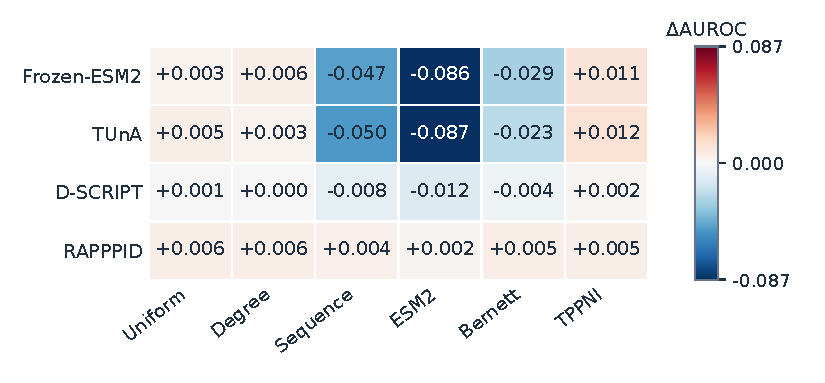
\includegraphics[width=\textwidth]{figure_pair_dependence_heatmap.pdf}
  \caption{\textbf{Effect of breaking the original protein pairs.} Each cell
  shows $\Delta$AUROC = AUROC(original pairs) $-$ AUROC(shuffled pairs).
  Positive values mean the original pairing gives a higher score; negative
  values mean shuffling gives a higher score. Values are means over seeds 11,
  22, and 33. The control only tests these evaluation sets and does not show
  that a model never uses pair-specific information.}
  \label{fig:pairdependence}
\end{figure*}

For Frozen-ESM2 and TUnA on the Sequence- and ESM-matched test sets, the
observed score does not require the original pair association. This does not
show that the models ignore their partner in general, and it does not identify
a molecular mechanism.

\subsection{Training-negative choice affects measured-assay performance}

On Vidal/Y2H, D-SCRIPT AUROC ranges from 0.428 to 0.574,
Frozen-ESM2 from 0.477 to 0.620, and TUnA from 0.454 to 0.623 across the six
training-negative constructions. RAPPPID varies less, from 0.480 to 0.533.
On IntAct, Frozen-ESM2 ranges from 0.424 to 0.581 and TUnA from 0.391 to 0.584;
the latter span is 0.193. These scores use the same external protein pairs and
differ only in the negative construction used to train the Gold models. The
complete model-by-construction matrix is shown separately for each measured
dataset in Figure~\ref{fig:measured-transfer}; each cell is a mean over the
three seeds.

\begin{figure*}[t]
  \centering
  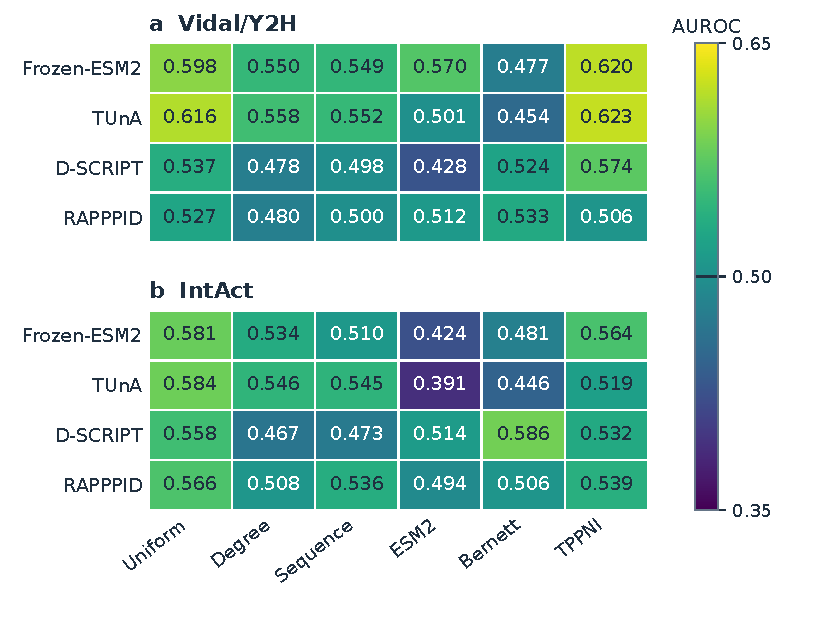
\includegraphics[width=\textwidth]{figure_measured_transfer_heatmaps.pdf}
  \caption{\textbf{Measured-assay performance changes with the Gold
  training-negative construction.} Vidal/Y2H and IntAct are shown separately.
  Columns are the six Gold training-negative constructions and rows are the
  four models, shown at left only. Values are absolute AUROC means over seeds
  11, 22, and 33; the shared color scale marks 0.5, the chance AUROC. The two
  panels are different datasets, not points along a trajectory. IntAct's class
  imbalance affects AUPRC, not the AUROC values shown here.}
  \label{fig:measured-transfer}
\end{figure*}

Because IntAct contains far more positives than negatives, we do not compare
its raw AUPRC directly with balanced Gold AUPRC. We report
prevalence-normalized and balanced diagnostics separately. This analysis tests
sensitivity to the training-negative construction; it does not treat either
assay as a universal ground truth.

\subsection{DataSAIL provides a separate leakage-control analysis}

The official DataSAIL analysis is supplementary because it changes the split
and the available sequence subset and includes only three of the four models.
It uses Uniform and ESM-matched negatives for both training and testing. Mean
AUPRC across its tested conditions is 0.529 for D-SCRIPT-ESM2, 0.582 for
Frozen-ESM2, and 0.584 for TUnA. This analysis tests split leakage in a reduced
two-construction setting and does not replace the main six-construction
experiment.

\section{Discussion}

A PPI benchmark score depends on how negatives are constructed. In our
experiments, changing the negative construction changes absolute performance,
model ordering, simple-control performance, dependence on the original pair,
and performance on measured datasets.

The partner-shuffling control shows why this matters. For some model/test-set
combinations, breaking the original A--B pairs leaves AUROC almost unchanged or
even increases it. This pattern is consistent with label-associated differences in individual
proteins or in the selected candidate pairs contributing to the score. Binary
benchmark performance alone is therefore not enough to show that a model
learned pair-specific interaction information.

Reducing one shortcut also does not guarantee higher measured-assay
performance. On the Bernett test set, the easy-property classifier is close to
chance (AUROC 0.514), but Bernett training does not consistently give the
highest Vidal or IntAct AUROC among the six training constructions. With TPPNI
training, Frozen-ESM2 and TUnA reach 0.620 and 0.623 AUROC on Vidal/Y2H, while
the TPPNI test set remains separable by the single-protein and pooled-ESM
controls (AUROC 0.648 and 0.669). Shortcut reduction, benchmark difficulty,
pair dependence, and measured-assay performance should therefore be reported
separately.

For studies that use constructed negatives, we recommend stating exactly how
negatives are generated and which protein pairs are eligible. At least one
alternative negative construction and simple pair-breaking controls should be
reported. Measured assay outcomes should remain separate from synthetic
unobserved pairs, and dataset shift should be distinguished from strict
protein/family separation from training. These checks make clear which
conclusions depend on the negative construction.

\section{Limitations}

The common 512-residue subset is needed to evaluate all four models under the
same sequence-length constraint, but it retains only 16.3\% of the original
Gold training positives. Results on this subset may not hold for the full Gold
release.

Most Gold negatives are synthetic unobserved pairs, not experimentally verified
non-interactions. Vidal/Y2H non-detections are assay outcomes and can contain
false negatives; IntAct negatives are context-specific curated evidence. None
of these labels supports the statement that two proteins can never interact.

The shortcut controls cover selected observable features and cannot rule out
all shortcuts. Partner shuffling tests whether the original pair is needed for
the observed score; it does not identify what biological mechanism, if any, a
model has learned. Three training seeds measure optimization variability rather
than biological replication. Several models also use pretrained protein
representations, so a protein-disjoint downstream split does not imply that the
representation model had no prior exposure to related PPI information
\citep{szymborski2026}.

\subsection*{Reproducibility statement}

The submission package records evaluation-set and checkpoint hashes, exact
seeds, fixed experiment configurations, validation-only selection rules,
sampler and model fidelity audits, machine-readable CSV/JSON data for every
main figure, and machine-readable main, external, and DataSAIL results. The
final experiment contains 72 trained model instances, 432 Gold evaluations,
576 external evaluation rows, 36 DataSAIL evaluations, and 510 control
results. The anonymized code package includes
the scripts used for data generation, training, scoring, analysis, and figures.

\subsection*{Ethics statement}

This work uses public protein sequence and interaction data and contains no
personal or clinical data. A risk is misreading a constructed negative as
evidence that two proteins cannot interact, or treating benchmark performance
as direct evidence of a molecular mechanism. We therefore keep each negative
label tied to its source and state which dataset each transfer or OOD claim
refers to.

\subsection*{AI use statement}

Generative AI tools were used for literature search and summarization,
methodological critique, software drafting and code review, analysis and figure
code, and manuscript drafting and editing. AI-assisted text and code were
checked against primary literature, repository code, fixed protocols, and
executed result files. Numerical claims were checked against the machine-readable figure data and
result summaries. The authors take responsibility for the
final methods, software, analyses, figures, and text.

\bibliography{references}
\bibliographystyle{iclr2027_conference}

\appendix

\section{Additional result details}

\paragraph{Execution summary.}
The final protocol completed all planned main evaluations: four
models, six training-negative constructions, six test-negative constructions,
and three seeds. External datasets are scored without retraining. The official
DataSAIL analysis is reported separately from the main Gold experiment.

\paragraph{IntAct prevalence.}
The IntAct set contains 10,111 positives and 236 explicit negatives. Because
positives dominate this set, its raw AUPRC is not compared to the 1:1 Gold
AUPRC. We also report a fixed balanced subset as a post-hoc sensitivity check.

\paragraph{Model-order reversals.}
The reversal analysis separates changes in point estimates from changes also
supported by paired evaluation resampling and seed-to-seed consistency. The
main text reports both counts.

\paragraph{DataSAIL.}
The official split uses its own dataset definition and sequence-compatibility
filter.
RAPPPID was not run in this analysis and is not imputed.

\section{Negative-construction characterization}

\begin{figure*}[t]
  \centering
  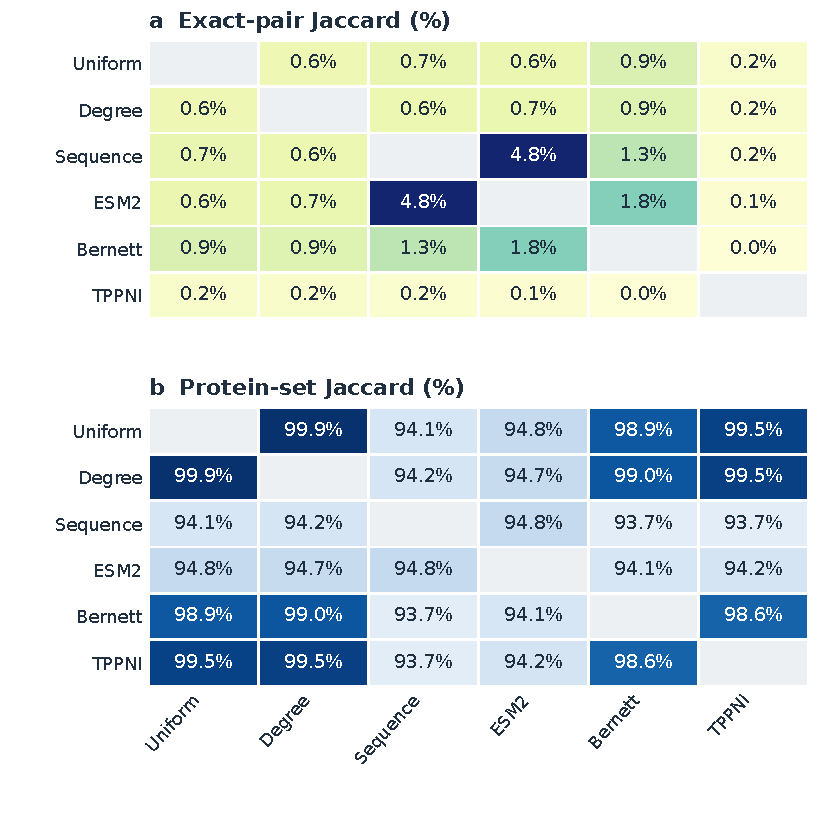
\includegraphics[width=\textwidth]{figure_negative_construction_characterization_main.pdf}
  \caption{Pairwise Jaccard overlap among the six Gold test-negative
  constructions. Exact unordered-pair overlap and protein-set overlap are shown
  separately as percentages, with diagonal cells omitted. Train-visible degree
  is degenerate on this protein-disjoint test cohort and remains a diagnostic.
  These set summaries are descriptive; overlap does not establish that one
  construction is more biologically realistic than another.}
  \label{fig:construction-overlap}
\end{figure*}

\begin{figure*}[t]
  \centering
  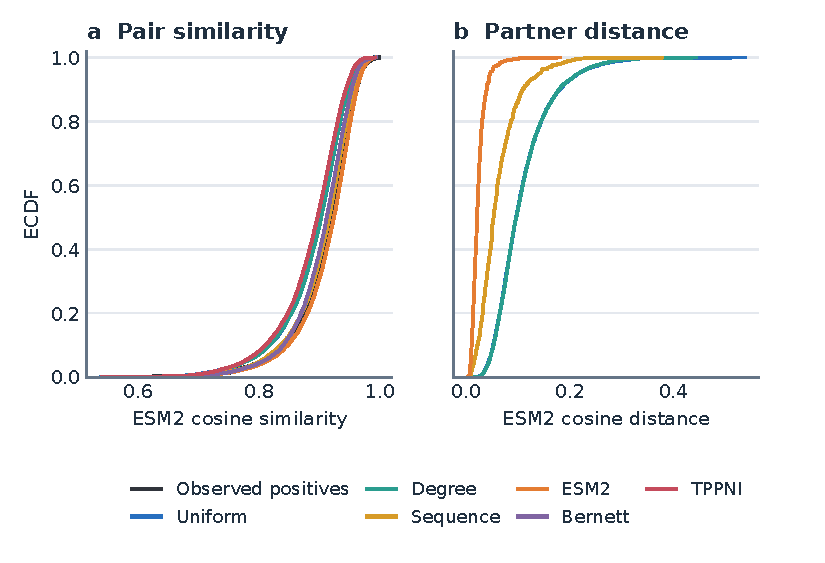
\includegraphics[width=\textwidth]{figure_negative_construction_characterization_ecdf.pdf}
  \caption{Frozen-input characterization of negative constructions. Left:
  empirical distributions of pair cosine similarity in ESM2 space for observed
  positives and all six test-negative constructions; ESM2 matching is expected
  to affect this representation-space quantity by design. Right: cosine
  distance between selected negative partners and observed partners for the
  four anchor-fixed constructions only; the global Bernett and TPPNI
  constructions do not define this anchor correspondence. These summaries are
  not PPI probabilities or evidence that constructed pairs are biological
  non-interactions.}
  \label{fig:construction-similarity}
\end{figure*}

\section{Artifact map}

The scientific summary, reviewer red-team, and claim ledger are included in the
repository. Original figure data and paper-specific figure data are stored
separately. Large run-level result registries are stored outside Git by project
policy; their hashes are recorded in the audit, and the values used in the paper
are included in committed machine-readable figure files.

\end{document}
